\documentclass[conference]{IEEEtran}
%\IEEEoverridecommandlockouts
% The preceding line is only needed to identify funding in the first footnote. If that is unneeded, please comment it out.
\usepackage[spanish]{babel}
\usepackage[utf8]{inputenc}
\usepackage{cite}
\usepackage{amsmath, amsthm,amssymb,amsfonts}
\usepackage{algorithmic}
\usepackage{graphicx}
\usepackage{textcomp}
\usepackage{xcolor}
\def\BibTeX{{\rm B\kern-.05em{\sc i\kern-.025em b}\kern-.08em
    T\kern-.1667em\lower.7ex\hbox{E}\kern-.125emX}}

% Definición del entorno 'definition'
\newtheorem{definition}{Definición}

\begin{document}

\title{Análisis de estabilidad para sistemas con retardos: Casos de aplicación práctica\\
	% {\footnotesize \textsuperscript{*}Note: Sub-titles are not captured in Xplore and
	% should not be used}
	% \thanks{Identify applicable funding agency here. If none, delete this.}
}

\author{
	\IEEEauthorblockN{José Alejandro León Sánchez}
	\IEEEauthorblockA{\textit{Posgrado de Ingeniería} \\
		\textit{UNAM}\\
		CDMX, Mexico}
	\and
	\IEEEauthorblockN{Martha Belem Saldívar Márquez}
	\IEEEauthorblockA{\textit{CINVESTAV} \\
		\textit{IPN}\\
		CDMX, Mexico}
}

\maketitle

\begin{abstract}
	Este documento es un resumen de la tercera ponencia del Seminario de Investigación de la Maestría en Ingeniería Eléctrica (Especialización en Control) del programa de Posgrado en Ingeniería de la UNAM, presentada por la Dra. Belem Saldivar. La ponencia abordó el análisis de estabilidad en sistemas con retardos, presentando tanto los fundamentos teóricos como aplicaciones prácticas. Se discutieron dos casos de estudio: el control de vibraciones en sistemas de perforación de pozos petroleros y el análisis de estabilidad en procesos de mecanizado con torno, destacando las herramientas y técnicas utilizadas para enfrentar los desafíos asociados con los retardos en dichos sistemas.
\end{abstract}

\begin{IEEEkeywords}
	Control robusto, Funciones multivaluadas, Inclusiones diferenciales, Monotonía, Modos deslizantes, Discretización implícita, Discretización explícita, Control multivaluado
\end{IEEEkeywords}


\section{Introducción}

Los sistemas con retardos aparecen comúnmente en diversas disciplinas como la ingeniería, biología y química, especialmente en aquellos que involucran transporte de materia o información. Estos retardos, aunque presentes en muchos sistemas, no siempre son significativos, pero cuando lo son, requieren una modelación adecuada para garantizar la estabilidad y el correcto funcionamiento del sistema.

Un ejemplo cotidiano de un sistema con retardo es el control de la temperatura del agua al ducharse. El ajuste de las llaves de agua caliente y fría no tiene un efecto inmediato, sino que se siente tras algunos segundos o minutos, lo cual ejemplifica el comportamiento típico de los sistemas con retardos.

Los sistemas con retardos se describen comúnmente mediante ecuaciones diferenciales del tipo:

\begin{equation}
	\dot{x}(t) = -x(t - \tau), \quad \tau > 0
\end{equation}

Una de las diferencias fundamentales con respecto a los sistemas sin retardos es que la condición inicial en sistemas con retardos incluye un segmento de trayectoria, en lugar de un valor puntual (Fig. \ref{fig:ci_retardos}). Además, el número de raíces del sistema es infinito, lo que complica su análisis en comparación con los sistemas sin retardo.

\begin{figure}[h]
	\centering
	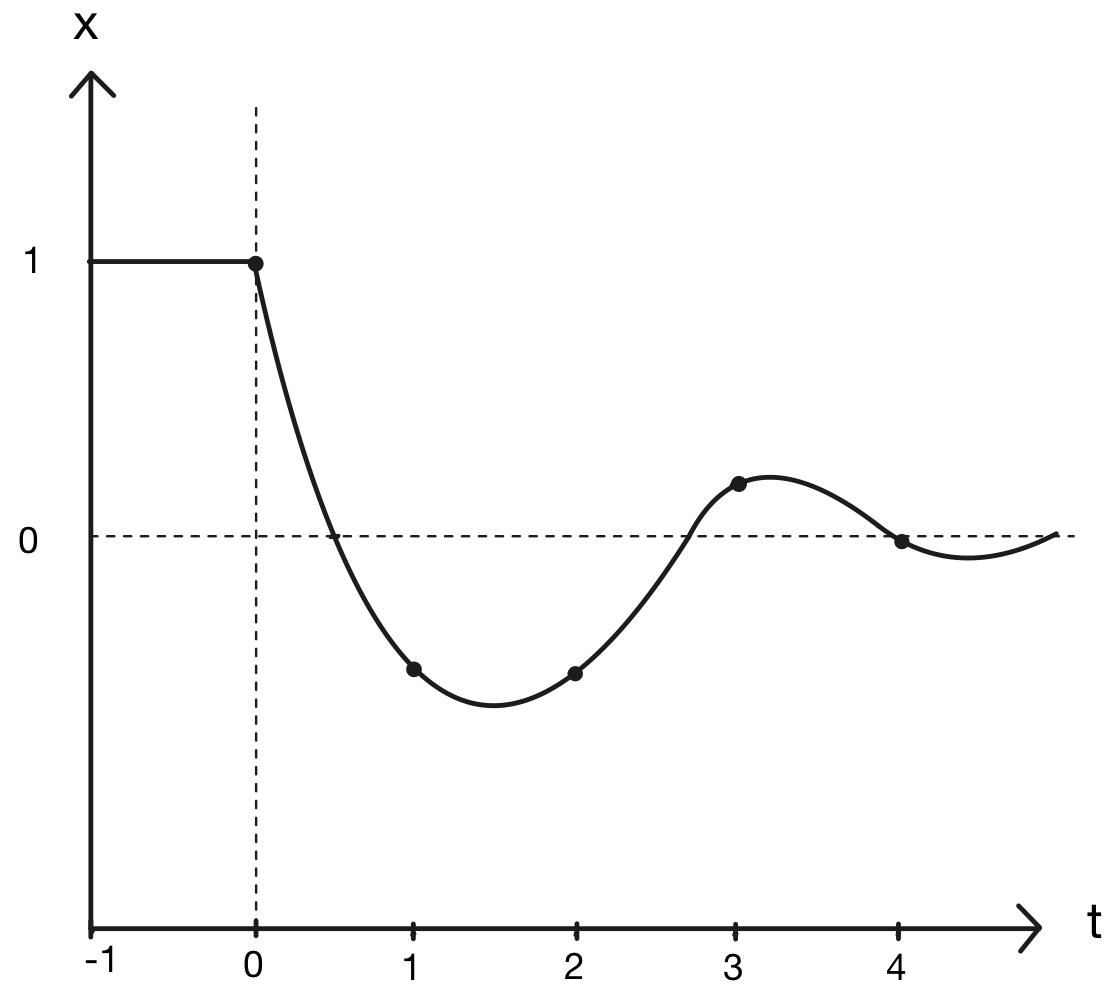
\includegraphics[width=0.3\textwidth]{ci.jpeg}
	\caption{Condición inicial en sistemas con retardos}
	\label{fig:ci_retardos}
\end{figure}

\section{Estabilidad de sistemas con retardos}

Para un sistema lineal sin retardos, representado por:

\begin{equation}
	\dot{x}(t) = A x(t),
\end{equation}
la estabilidad puede determinarse a partir de la localización de las raíces del polinomio característico:

\begin{equation}
	p(s) = \det(sI - A) = a_0 s^n + a_1 s^{n-1} + \dots + a_{n-1} s + a_n,
\end{equation}
el cual tiene un número finito de raíces. Sin embargo, al introducir un retardo en el sistema, la ecuación diferencial se modifica de la siguiente manera:

\begin{equation}
	\dot{x}(t) = A_0 x(t) + A_1 x(t-h), \quad A_0, A_1 \in \mathbb{R}^{n \times n},
\end{equation}
donde \( h \) es el retardo. La estabilidad de este sistema se puede determinar a partir de las raíces del cuasipolinomio característico:

\begin{equation}
	p_h(s) = \det(sI - A_0 - A_1 e^{-sh}),
\end{equation}
dado que esta ecuación es trascendental, tiene un número infinito de soluciones.

Otra aproximación común para el estudio de la estabilidad es el uso de la teoría de Lyapunov. Para un sistema lineal sin retardos, la estabilidad se puede garantizar si existe una matriz \( P > 0 \) tal que la siguiente expresión se cumpla:

\begin{equation}
	A^T P + P A = -Q, \quad Q > 0,
\end{equation}
y, de esta forma, la derivada de la función de Lyapunov:

\begin{equation}
	\dot{V} = x^T(t) [A^T P + P A] x(t),
\end{equation}
es definida negativa.

En el caso de sistemas con retardos, la situación es más compleja. Si se considera la función de Lyapunov:

\begin{equation}
	V = x^T(t) P x(t), \quad P = P^T > 0,
\end{equation}
la derivada de esta función es:

\begin{equation}
	\begin{aligned}
		\dot{V} & = \dot{x}^T(t) P x(t) + x^T(t) P \dot{x}(t)                                                                \\
		        & = x^T(t) A_0^T P x(t) + x^T(t-h) A_1^T P x(t)                                                              \\
		        & \quad + x^T(t) P A_0 x(t) + x^T(t) P A_1 x(t-h)                                                            \\
		\dot{V} & = \begin{bmatrix} x^T(t) & x^T(t-h) \end{bmatrix} \bar{\Psi} \begin{bmatrix} x(t) \\ x(t-h) \end{bmatrix},
	\end{aligned}
\end{equation}
donde:

\begin{equation}
	\bar{\Psi} = \begin{bmatrix} P A_0 + A_0^T P & P A_1 \\ A_1^T P & 0 \end{bmatrix}.
\end{equation}

Dado que no se puede garantizar que \( \bar{\Psi} < 0 \), esta función de Lyapunov no es suficiente para analizar la estabilidad del sistema con retardo.

Para resolver esta dificultad, se puede utilizar la funcional de Lyapunov-Krasovskii, que toma la forma:

\begin{equation}
	V(t, x_t) = x^T(t) P x(t) + \int_{t-h}^{t} x^T(s) Q x(s) ds, \quad P > 0, Q > 0.
\end{equation}

Tomando la derivada de esta función

\begin{equation}
	\begin{aligned}
		\dot{V}(t, x_t) & = \dot{x}^T(t) P x(t) + x^T(t) P \dot{x}(t)                                                                  \\
		                & = x^T(t) A_0^T P x(t) + x^T(t-h) A_1^T P x(t)                                                                \\
		                & \quad + x^T(t) P A_0 x(t) + x^T(t) P A_1 x(t-h)                                                              \\
		                & \quad + x^T(t) Q x(t) - x^T(t-h) Q x(t-h)                                                                    \\
		\dot{V}(t, x_t) & = \begin{bmatrix} x^T(t) & x^T(t-h) \end{bmatrix} \bar{\Psi}_h \begin{bmatrix} x(t) \\ x(t-h) \end{bmatrix},
	\end{aligned}
\end{equation}
donde:

\begin{equation}
	\bar{\Psi}_h = \begin{bmatrix} P A_0 + A_0^T P + Q & P A_1 \\ A_1^T P & -Q \end{bmatrix}.
\end{equation}

Para garantizar la estabilidad asintótica del sistema con retardo, es necesario verificar que la matriz \( \bar{\Psi}_h \) sea definida negativa, es decir, que \( \bar{\Psi}_h < 0 \).

\section{Vibraciones en sistemas de perforación}

En los sistemas de perforación, la tubería que conecta la mesa giratoria con la broca puede adquirir propiedades elásticas debido a su longitud, lo que genera ondas torsionales. Un fenómeno común es el "stick-slip", donde la tubería se atora en un punto de la parte inferior mientras el extremo superior sigue girando, acumulando energía que, al liberarse, hace que la broca gire a velocidades mayores que la mesa giratoria.

Se modeló este fenómeno usando la ecuación de onda, manipulando la solución general mediante la transformación de D'Alambert para obtener una ecuación diferencial con retardos. Entre las estrategias prácticas mencionadas están la ley de variación del peso sobre la broca, el aumento del amortiguamiento y el diseño de control basado en Lyapunov-Krasovskii. Problemas abiertos incluyen la consideración de dinámicas acopladas y retardos variantes en el tiempo debido a la longitud cambiante de la barra.

\section{Estabilidad en procesos de mecanizado con torno}
En los sistemas de mecanizado, las vibraciones tienen efectos negativos que van desde la degradación de la calidad del acabado superficial hasta el desgaste acelerado de la herramienta, lo que eleva los costos operativos y reduce el rendimiento del proceso. Este fenómeno obliga a reducir las velocidades de corte para mitigar su impacto, lo que a su vez afecta la eficiencia. Además, las vibraciones pueden generar ruido excesivo y potencialmente dañar la máquina.

El objetivo principal de este estudio fue emplear técnicas tanto en el dominio del tiempo como en el de la frecuencia para sistemas con retardos, con el fin de determinar parámetros operativos que eviten las vibraciones en el mecanizado. A partir del modelado matemático, se presentó una ecuación diferencial con retardos, obteniéndose el cuasipolinomio característico para el análisis de estabilidad. Los parámetros clave son la velocidad de rotación y la profundidad de corte. Para el análisis, se utilizó el método de D-particiones, que ayuda a identificar regiones estables en el espacio de parámetros. Además, se presentaron controladores basados en la teoría de Lyapunov-Krasovskii para sistemas con retardos, buscando garantizar la estabilidad del proceso.

\section*{Conclusiones}

En conclusión, el análisis de estabilidad en sistemas con retardos, tanto en aplicaciones industriales como en procesos de perforación y mecanizado, es crucial para garantizar el funcionamiento seguro y eficiente. Las técnicas de control basadas en Lyapunov-Krasovskii y el uso de ecuaciones diferenciales con retardos permiten un análisis profundo de la dinámica involucrada, aportando estrategias prácticas para mitigar los efectos negativos, como las vibraciones. Sin embargo, persisten retos abiertos, como el manejo de las no linealidades y la extensión de estos análisis a otros procesos, lo que sigue siendo un campo fértil para futuras investigaciones.

\begin{thebibliography}{00}
	\bibitem{Saldivar2016}
	Saldivar, B., Mondié, S., et al. (2016). A control oriented guided tour in oilwell drilling vibration modeling. \textit{Annual Reviews in Control}, 42, 100-113.

	\bibitem{Castorena2024}
	Castorena-Minor, H., Saldivar, B. (2024). Critical depth of cut in turning processes: Time and frequency domain approaches. \textit{IFAC Workshop on Time Delay Systems}, Udine, Italia, Septiembre 2024.

	\bibitem{Ramirez2018}
	Ramírez, L. F., Saldivar, B., et al. (2018). Lyapunov-Krasovskii approach to the stability analysis of the milling process. \textit{IET Control Theory \& Applications}, 12(9), 2018.


\end{thebibliography}

\end{document}
